\documentclass[letterpaper,12pt]{article}

\usepackage[cm]{fullpage}					% To maximize spacing on letter paper
\usepackage{color}							% For pretty colors
\usepackage[pdftex]{graphicx}				% To import images
\usepackage{fancyhdr}						% Fancy Headers and Footers
\usepackage{parskip}						% Vertical spacing inbetween paragraphs

\newcounter{qcounter}						% For custom lists

\newcounter{rcounter}						% For counting in tabular environments
\newcommand\rnumber{\stepcounter{rcounter}\arabic{rcounter}}

% We are customizing the \Section command here so that all figures in each section
% follow the 'Figure s-n' convention, where 's' is the section number and 'n' is the
% nth figure in the section.
\renewcommand{\thefigure}{\thesection-\arabic{figure}}
\newcommand{\Section}[1]{\section{#1} \setcounter{figure}{0}}

\definecolor{section}{RGB}{54,95,145}
\definecolor{subsection}{RGB}{79,129,189}
\definecolor{subsubsection}{RGB}{79,129,189}
\definecolor{footer}{RGB}{191,191,191}

\raggedright								% Turn-off indentation default

\graphicspath{{./images/}}					% Set path for image files

\pagestyle{fancy}
\fancyhf{}									% Clear default header/footer
\renewcommand{\headrulewidth}{0pt}			% Remove default horizontal rule in header
\rfoot{\textcolor{footer}{\thepage}}		% Page Number
\lfoot{\textcolor{footer}{FRD/SDD/SID/TPD for IM-Net, by Aggrawal, Bogle, Kelsey and Ortega. Winter 2012.}}

\begin{document}

\tableofcontents
\listoffigures

\eject

{\textcolor{section}{\Section{Introduction}}

\textcolor{subsection}{\subsection{Purpose}}

The purpose of this document is four-fold:

\begin{enumerate}
\item  Define a full set of requirements for the IM-Net. (These sections correspond to a Software Requirements Document (SRD)).

\item  Define the design for the IM-Net. (These sections correspond to a Software Design Document (SDD)).

\item  Define the Test Plan for the IM-Net. (These sections correspond to a Software Test Plan (STP)).

\item  Define and partially implement feasible modules for the IM-Net.  (These sections correspond to the Software Implementation Document (SID)).
\end{enumerate}

The complete definition of all IM-Net requirements provides the source requirement inputs for the development of the subsequent supporting software subsystems documents.

\textcolor{subsection}{\subsection{Scope}}

The documentation developed as part of this CS437 class, starts from the SRD prepared in CS337 or in previous CS437 classes with a much reduced scope.  The scope of this document includes the following:

\begin{enumerate}
\item  All functional and non-functional requirements on the IM-Net are captured.  This includes Verification \& Validation (V\&V) requirements, as well as inter-software subsystems requirements.

\item  A complete set of IM-Net Requirements, derived and traceable to the incoming class requirements.  These requirements are organized by key IM-Net functional units shown on the Level 1 DFD given in section 2.0.

\item  A trace matrix, relating all IM-Net functional requirements to functional subunits as expanded in lower level DFDs. Higher level DFDs are provided as part of the design in section 4.0

\item  The functional requirements defined in the IM-Net Requirements section have been expanded to include more specific hardware requirements.
\end{enumerate}

\textcolor{subsubsection}{\subsubsection{Organization}}

The organization of this document provides a natural 'flow' or allocation of requirements to each succeeding section. Details regarding the overall document structure are discussed in sub-section 1.4.

\textcolor{subsubsection}{\subsubsection{Relationship to Other Documents}}

The IM-Net SRD/SDD/STP/SID is a complete self contained document. Some relationships to other documents in the literature are indicated below in sub-section 1.5.

\textcolor{subsection}{\subsection{Project Name Architecture}}
 
\textcolor{subsubsection}{\subsubsection{Detailed Context Diagram (DFD Level 0)}}

The IM-Net architecture is summarized in the Context Diagram (DFD Level 0) given below. A more detailed Functional Description is given in Section 2 of this document.\\

\begin{figure}[h]
\centering
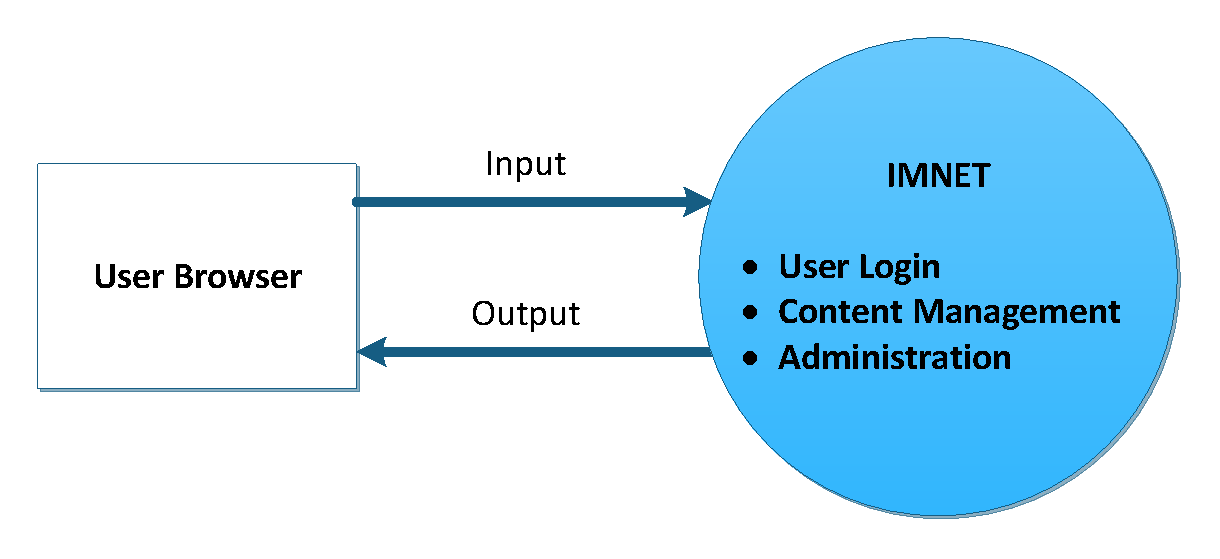
\includegraphics[scale=0.9]{DFD_level_0.pdf}
\caption{Context Diagram (DFD Level 0)}
\label{fig:DFD_level_0}
\end{figure}

The foremost objective of IM-Net is to assist music artists, label and venues in reaching out to their fans through a vibrant, web-based, multimedia interface.

IM-Net is a software application which provides major functions such as the ones listed below:

\begin{enumerate}
\item  Provides a portal for independent music artists, labels and venues to connect with their fans.

\item  The ability for artists and label to upload and showcase their music to their fans.

\item  Allows music artists, labels and venue to connect to their fans through the messaging interface.
\end{enumerate}

IM-Net is implemented primary using the Django content management system, a web-based framework that closely follows the Model-View-Controller architectural pattern. Data models are framed using Python classes and are stored into a SQL relational database. Views are implemented using Django's Template language, which are used by Django to generate dynamic HTML output. Controllers are Python scripts that describe to the view which particular data will be shown. 

TODO: WRITE MORE HERE

\textcolor{subsection}{\subsection{Documentation Development Process}}

The IM-Net detailed functional description is documented in section 2.0. Basically, Section 2 is a succinct software description document. The overall detailed functional description is based on higher level DFDs (above level 1). All major functional units are described in detail in this part of the document.

Requirements affecting the IM-Net are captured in Section 3.0 of this document.  These requirements are a refinement and completion of requirements first collected as part of a previous Software Engineering project. The document is cited in Section 1.2.2. This section is the one worked in most detail to become a reasonably complete Software Requirements Document (SRD). It includes both functional and non-functional software requirements together with several detailed ``rational'' paragraphs whenever necessary to complete the understanding of each requirement.

Section 4 is the IM-Net detailed Design Description Document (SDD). This part of the document includes all higher level DFDs as described in section 2 plus all interface units. The document is highly technical and it is based on section 2 descriptions. An important component is the addition of a SIS (software interface specification) document in sub-section 4.2.

Section 5 includes elements of a partial implementation of the IM-Net. This section includes the various constraints that effectively limit the implementation as well as the sub-units that will be coded. The implementation goals are defined and the code and pseudo code are included as an attachment to this section.  

Section 6 is the last major section in this document and includes the overall Test Plan (TP) of the IM-Net. The test plan details the various techniques used to test the requirements and it also includes a Validation Matrix where each requirement specified in section 3 is listed with its corresponding validation method. In addition, TP specifies the mandated peer reviews needed to validate the stakeholders part of the requirements.

 
\textcolor{subsection}{\subsection{References}}

All references used in the creation of this document are listed below.

\textcolor{subsubsection}{\subsubsection{Controlling Documents}}

There is no document controlling this document.

\textcolor{subsubsection}{\subsubsection{Applicable Documents}}

No addition applicable document has been used in the production of this document.

\textcolor{subsection}{\subsubsection{Standards}}

No Standard has been used in the creation of this document. However, some Standards described in textbooks have been examined as a reference. In particular, the IEEE standard has been briefly discussed in class.

\eject

\textcolor{section}{\Section{Detailed Function Description of IM-Net}}

\textcolor{subsection}{\subsection{Detailed IM-Net Functional Description}}

\textcolor{subsubsection}{\subsubsection{High Level DFDs}}

The IM-Net major functional subunits are shown in the DFD Level 1 depicted below:

\begin{figure}[h!]
\centering
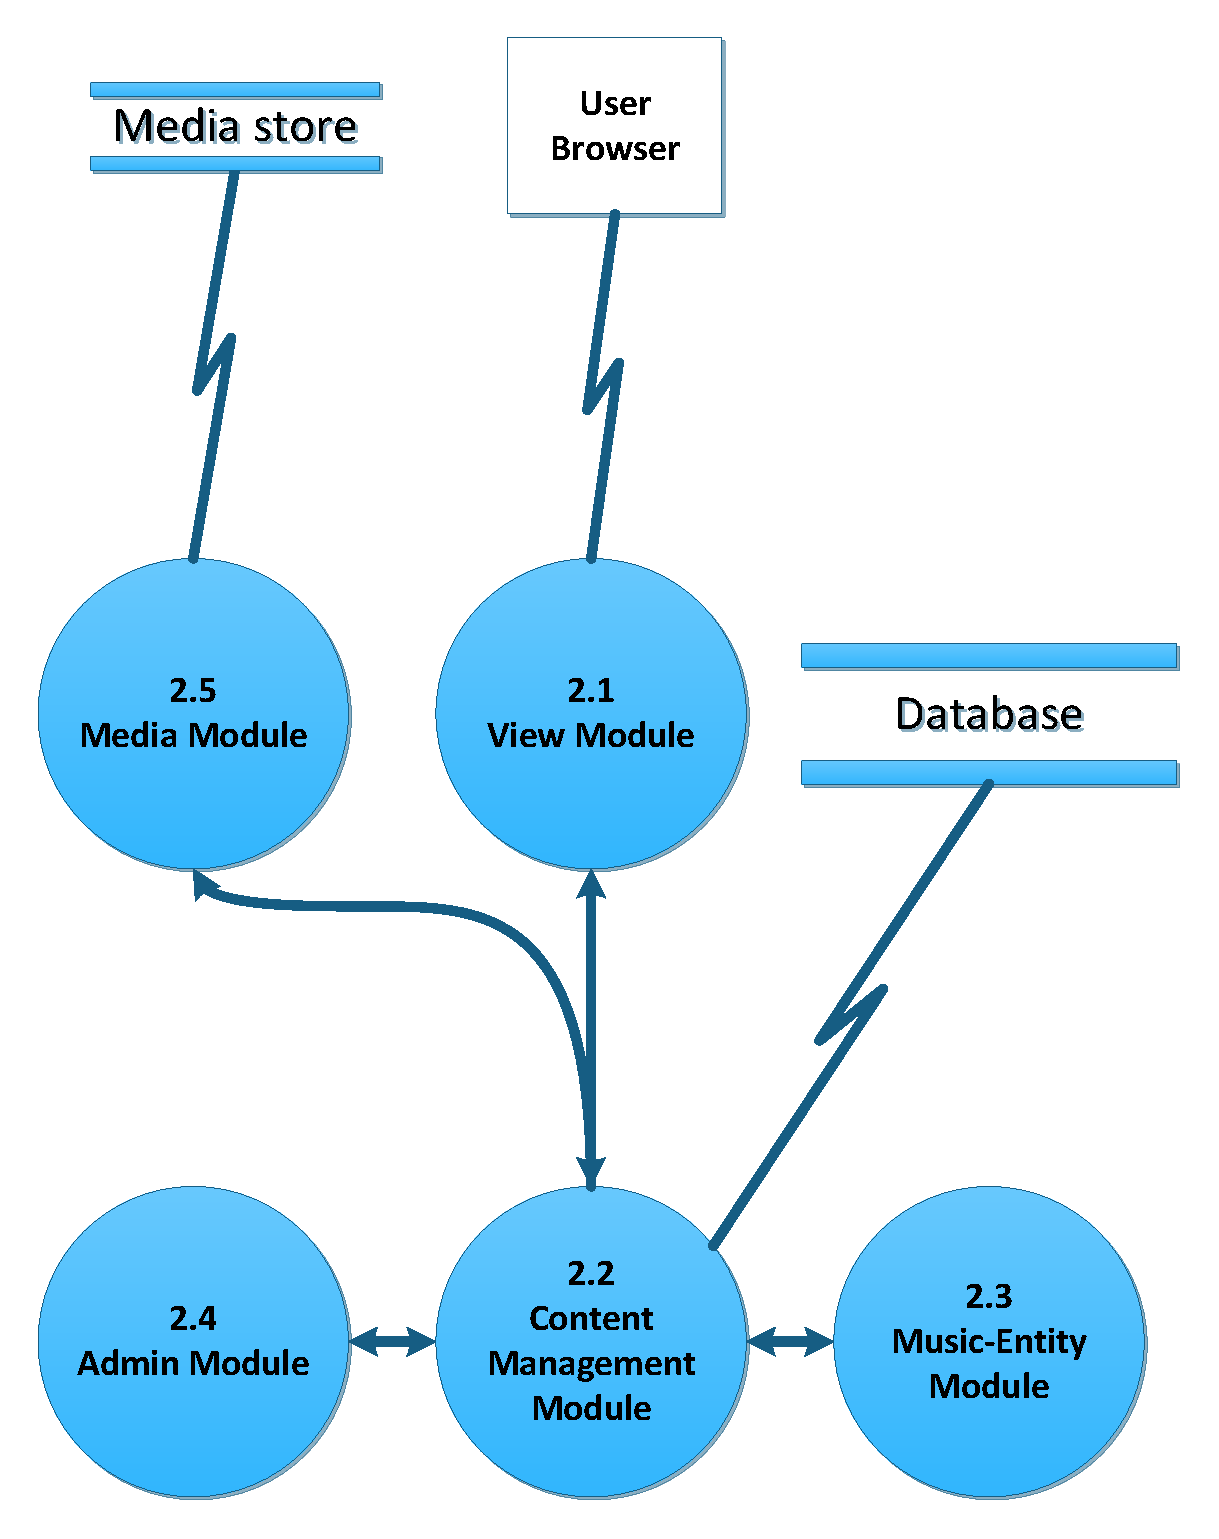
\includegraphics[scale=0.6]{DFD_level_1.pdf}
\caption{DFD Level 1}
\label{fig:DFD_level_1}
\end{figure}
 
\textcolor{subsubsection}{\subsubsection{Detailed Functional Description of the IM-Net Major Units}}

The description of the function of the IM-Net major functional units shown in Figure \ref{fig:DFD_level_1} follows.

\paragraph{View - Module 2.1}
The View module is responsible for communicating with the user's browser and generating the client-side appearance and functionality of IM-Net.

\paragraph{Content Management - Module 2.2}
The Content Management module is the interface hub between all other IM-Net modules and the database. All IM-Net data are framed within the Content Management module using the pre-defined Python classes, then stored in the database. The Controller function receives all requests from the View module, gets the appropriate data from the database and other modules, and send the response back to the View module. The Registration function handles all registration requests by creating new user information and permissions in the database, then e-mails the new user their login information. The User-Authentication function handles login requests, querying the database for the proper credentials, and if successful, returns the user's proper permissions. The Messaging function handles all IM-Net internal messaging , i.e., tracking intercommunication in between all IM-Nets users through message threads.

\paragraph{Music-Entity - Module 2.3}
The Music-Entity module provides the Music-Entity abstract superclass that all artists, labels and venues classes are framed upon.

\paragraph{Administration - Module 2.4}
The Administration module provides the super-user interface for all IM-Net administrators.

\paragraph{Media - Module 2.5}
The Media module handles the safe storage of all IM-Net media files in the IM-Net Media Store.


\eject

\textcolor{section}{\Section{The IM-Net Requirements}}
 
\textcolor{subsection}{\subsection{IM-Net Functional Requirements}}

This Section collects all the IM-Net Functional Requirements. This section includes the complete set of functional requirements with explanation and rational where the statement of the requirement was deemed insufficient or needing additional background/justification. All requirements relate to the design modules described in Section 2. An effort has been made to standardize the correlation between the design modules and the requirements to make their access and organization more consistent. For example, requirement number ``n'' affecting module 2.1 will be labeled 3.1-n.

\setcounter{rcounter}{0}

\begin{center}
\begin{tabular}{|l|p{6in}|}
\hline 
\multicolumn{2}{|c|}{\textbf{Requirements Related to Design Module 2.1: View}} \\ 
\hline 
Requirement No. & Requirement Description \\ 
\hline
& \textbf{Web-Server Daemon:} \\
\hline
\textbf{3.1-\rnumber} & IM-Net shall run a web-server daemon to interface with the user's browser. \\ 
\hline 
\textbf{3.1-\rnumber} & IM-Net web-server daemon shall route all requests to the Content Management controller function. \\ 
\hline 
\textbf{3.1-\rnumber} & IM-Net web-server daemon shall route all responses to the user's browser. \\ 
\hline  
& \textbf{Templates:} \\
\hline
\textbf{3.1-\rnumber} & IM-Net HTML templates shall conform with the XHTML 1.0 Transitional standard set by the W3C. \\ 
\hline 
\textbf{3.1-\rnumber} & IM-Net CSS templates shall conform with the CSS level 3 standard set by the W3C. \\ 
\hline 
\textbf{3.1-\rnumber} & IM-Net shall store all template files on the server's local filesystem. \\
\hline
\textbf{3.1-\rnumber} & IM-Net shall have a base template. \\ 
\hline 
\textbf{3.1-\rnumber} & IM-Net shall have a base artist template. \\ 
\hline 
\textbf{3.1-\rnumber} & IM-Net shall have a base label template. \\ 
\hline 
\textbf{3.1-\rnumber} & IM-Net shall have a base venue template. \\ 
\hline 
\textbf{3.1-\rnumber} & IM-Net shall have a base fan template. \\ 
\hline 
\textbf{3.1-\rnumber} & IM-Net shall have a base messaging template. \\ 
\hline 
& \textbf{Interpreter:} \\
\hline
\textbf{3.1-\rnumber} & IM-Net shall generate dynamic HTML/CSS code using data from the Content Management Controller and the pre-defined template files. \\ 
\hline 
\textbf{3.1-\rnumber} & IM-Net shall route all dynamically generated HTML/CSS to the Web-Server daemon. \\ 
\hline 

\end{tabular} 
\end{center}

\setcounter{rcounter}{0}
\begin{center}
\begin{tabular}{|l|p{6in}|}
\hline 
\multicolumn{2}{|c|}{\textbf{Requirements Related to Design Module 2.2: Content Management}} \\ 
\hline 
Requirement No. & Requirement Description \\ 
\hline
& \textbf{Controller:} \\
\hline
\textbf{3.2-\rnumber} & IM-Net shall query the database for all data requests. \\ 
\hline 
\textbf{3.2-\rnumber} & IM-Net shall send all request data to the Interpreter function in the View module. \\
& \textbf{Rationale:} IM-Net generates all dynamic content by parsing the template files and inserting the appropriate data using the Interpreter function. \\
\hline 
& \textbf{Registration:} \\
\hline
\textbf{3.2-\rnumber} & IM-Net shall receive user registration requests. \\
\hline 
\textbf{3.2-\rnumber} & IM-Net shall write user registration information to the database. \\ 
\hline 
\textbf{3.2-\rnumber} & IM-Net shall not allow new users access until a validation check is complete. \\ 
\hline 
\textbf{3.2-\rnumber} & IM-Net shall perform user registration validations through e-mail. \\
& \textbf{Rationale:} To ensure that the new user's e-mail address is a actual existing e-mail address.\\
\hline 
\textbf{3.2-\rnumber} & IM-Net validation e-mails shall include a click-back link to IM-Net. \\ 
\hline 
\textbf{3.2-\rnumber} & IM-Net shall immediately allow users access once the validation check is complete. \\ 
\hline 
\textbf{3.2-\rnumber} & IM-Net shall encrypt all user passwords. \\ 
\hline 
\textbf{3.2-\rnumber} & IM-Net shall encrypt all user e-mail addresses. \\ 
\hline 
& \textbf{User Authentication:} \\
\hline
\textbf{3.2-\rnumber} & IM-Net shall verify all authentication information against the proper username/password combination stored in the database. \\ 
\hline 
\textbf{3.2-\rnumber} & IM-Net shall authenticate users before allowing access to the messaging interface. \\ 
\hline 
\textbf{3.2-\rnumber} & IM-Net shall authenticate users before allowing access to the fan interface. \\ 
\hline 
\textbf{3.2-\rnumber} & IM-Net shall authenticate user before allowing users to define favorite artists. \\ 
\hline 
\textbf{3.2-\rnumber} & IM-Net shall authenticate user before allowing users to define favorite labels. \\ 
\hline 
\textbf{3.2-\rnumber} & IM-Net shall authenticate user before allowing users to define favorite venues. \\ 
\hline 
& \textbf{Messaging:} \\
\hline
\textbf{3.2-\rnumber} & IM-Net shall allow all users to communicate with each other through a built-in messaging interface. \\ 
\hline 
\textbf{3.2-\rnumber} & IM-Net messaging interface shall include a inbox that contains all messages that have been sent to the user. \\ 
\hline 
\textbf{3.2-\rnumber} & IM-Net messaging interface shall include a sent messages folders that contains all messages that the user has sent to other users.  \\ 
\hline 
\textbf{3.2-\rnumber} & IM-Net messaging interface shall include a deleted messages folder that contains all messages that have been recently deleted by a user. \\ 
& \textbf{Rationale:} To allow the user to access a message that may have been invertenly deleted. \\
\hline 
\textbf{3.2-\rnumber} & IM-Net messaging interface shall allow all messages to have a subject line. \\ 
\hline 
\textbf{3.2-\rnumber} & IM-Net messaging interface shall allow all messages to have a message body.  \\ 
\hline 



\end{tabular} 
\end{center}

\setcounter{rcounter}{0}
\begin{center}
\begin{tabular}{|l|p{6in}|}
\hline 
\multicolumn{2}{|c|}{\textbf{Requirements Related to Design Module 2.3: Music-Entity}} \\ 
\hline 
Requirement No. & Requirement Description \\ 
\hline
& \textbf{Music-Entity Super-class:} \\
\hline
\textbf{3.3-\rnumber} & IM-Net shall store the name of each Music-Entity. \\ 
\hline
\textbf{3.3-\rnumber} & IM-Net shall store unique short-name of each Music-Entity. \\ 
\hline 
\textbf{3.3-\rnumber} & IM-Net shall store a description of each Music-Entity. \\ 
\hline 
\textbf{3.3-\rnumber} & IM-Net shall store a owner based upon a unique IM-Net user for each Music-Entity. \\ 
\hline 
\textbf{3.3-\rnumber} & IM-Net shall store all fans based upon IM-Net users for each Music-Entity. \\ 
\hline 
\textbf{3.3-\rnumber} & IM-Net shall store a musical genre for each Music-Entity \\ 
\hline 
\textbf{3.3-\rnumber} & IM-Net shall store a HTTP-based URL to a Music-Entity's owner preferred web-site for each Music-Entity. \\ 
\hline
\textbf{3.3-\rnumber} & IM-Net shall store a image file for each Music-Entity. \\ 
\hline
& \textbf{Music-Entity Sub-classes:} \\
\hline
\textbf{3.3-\rnumber} & IM-Net shall store each Artist Music-Entity that belongs to a Label Music-Entity. \\ 
\hline 
\textbf{3.3-\rnumber} & IM-Net shall store a location for each Venue Music-Entity. \\ 
\hline 
\textbf{3.3-\rnumber} & IM-Net shall store date-specific events for each Venue/Artist(s) Music-Entity relationship. \\ 
\hline
\textbf{3.3-\rnumber} & IM-Net shall  \\ 
\hline 
\textbf{3.3-\rnumber} & Requirement \\ 
\hline 
\textbf{3.3-\rnumber} & Requirement \\ 
\hline 

\end{tabular} 
\end{center}

\setcounter{rcounter}{0}
\begin{center}
\begin{tabular}{|l|p{6in}|}
\hline 
\multicolumn{2}{|c|}{\textbf{Requirements Related to Design Module 2.4: Administration}} \\ 
\hline 
Requirement No. & Requirement Description \\ 
\hline
\textbf{3.4-\rnumber} & Requirement \\ 
\hline 
\end{tabular} 
\end{center}

\setcounter{rcounter}{0}
\begin{center}
\begin{tabular}{|l|p{6in}|}
\hline 
\multicolumn{2}{|c|}{\textbf{Requirements Related to Design Module 2.5: Media}} \\ 
\hline 
Requirement No. & Requirement Description \\
\hline
& \textbf{Media Store:} \\
\hline
\textbf{3.5-\rnumber} & IM-Net shall store all media files into the Media Store based upon a hierarchical Artist/Album structure. \\ 
\hline
\textbf{3.5-\rnumber} & IM-Net Media Store shall be based upon a hierarchical Artist/Album structure. \\ 
\hline
\textbf{3.5-\rnumber} & IM-Net shall store all Media Store files into a redundant file-system. \\ 
\hline
\textbf{3.5-\rnumber} & IM-Net shall delete all media files in the Media Store requested to be deleted by the media file owner. \\ 
\hline
\textbf{3.5-\rnumber} & IM-Net shall ensure that no duplicate media files exist in the Media Store. \\ 
\hline
\textbf{3.5-\rnumber} & IM-Net shall ensure that all uploaded media files are limited to the MPEG-1 or MPEG-2 Audio Layer III standard (MP3). \\ 
\hline
\textbf{3.5-\rnumber} & IM-Net shall ensure that all uploaded media files are tagged with title metadata. \\ 
\hline
\textbf{3.5-\rnumber} & IM-Net shall ensure that all uploaded media files are tagged with artists metadata. \\ 
\hline
\textbf{3.5-\rnumber} & IM-Net shall ensure that all uploaded media file artist tags match the user's Music-Entity name. \\ 
\hline
\textbf{3.5-\rnumber} &  \\ 
\hline
\textbf{3.5-\rnumber} &  \\ 
\hline
& \textbf{Security:} \\
\hline
\textbf{3.5-\rnumber} & IM-Net shall check every uploaded media file for malicious code using anti-virus software. \\ 
\hline
\textbf{3.5-\rnumber} & IM-Net shall perform anti-virus database updates daily.\\ 
\hline
\textbf{3.5-\rnumber} & IM-Net shall disable media uploads if anti-virus updates cannot be completed as scheduled. \\ 
\hline 
\textbf{3.5-\rnumber} & IM-Net shall re-enable media uploads when disabled if anti-virus updates are completed. \\ 
\hline
\textbf{3.5-\rnumber} & IM-Net shall immediately quarantine and delete any media file uploads indentified by the anti-virus as compromised by malicious code. \\ 
\hline
\textbf{3.5-\rnumber} & IM-Net shall notify the user if any media file uploads are indentified by the anti-virus as compromised by malicious code. \\ 
\hline
\textbf{3.5-\rnumber} & Requirement \\ 
\hline
\textbf{3.5-\rnumber} & Requirement \\ 
\hline
\textbf{3.5-\rnumber} & Requirement \\ 
\hline
\end{tabular} 
\end{center}

\textcolor{subsection}{\subsection{IM-Net Non-Functional Requirements}}

This Section collects all the IM-Net Non-Functional Requirements. All non-functional requirements are numbered ``NF -- n'' where ``n'' indicates the n${}^{th}$ requirement.

\begin{list}{NF -- \arabic{qcounter}:~}{\usecounter{qcounter}}

\item  IM-Net shall require minimal training for users who have experience with common web browsers and web-based applications.

\item  IM-Net shall not disclose any personal information about any artists, label, venue or fan to unauthorized users.

\item  IM-Net shall be deployable to any Apache/SQL/Python/Django software stack within 5 hours of unpacking the IM-Net software package.

\end{list}

\textcolor{subsection}{\subsection{IM-Net Hardware Requirements}}

This Section collects all the IM-Net Hardware Requirements. All hardware requirements are numbered ``H -- n'' where ``n'' indicates the n${}^{th}$ requirement.

\begin{list}{H -- \arabic{qcounter}:~}{\usecounter{qcounter}}

\item  IM-Net requires a redundant and scalable compute cloud instance.

\item  The IM-Net computer cloud instance requires 99.99\% uptime through a proper environmentally controlled and power redundant data center.

\end{list}

\eject

\textcolor{section}{\Section{IM-Net Detailed Design}}

In this section, the IM-Net described in Section 2 with requirements listed in Section 3 will be designed in detail including several higher level DFDs. Each major module detailed design is included in correspondence with the design sections defined in Section 2 and responding to the requirements listed in its correlated sub-section in chapter 3.

The detailed design of each of the four modules discussed in section 2 with requirements presented in section 3 is presented in Figures 4-1, 4-2, 4-3, and 4-4. As done in previous cases, Figure 4-1 corresponds to the detailed design of Module 2.1, and so on.

Figure 4-1 shows the four sub-modules that comprise module 2.1. Next, Figure 4-2 shows the three sub-modules that comprise module 2.2. Then, Figure 4-3 shows the four sub-modules that comprise module 2.3. Lastly, Figure 4-4 depicts the three sub-modules that comprise module 2.4.

\begin{figure}[h!]
\centering
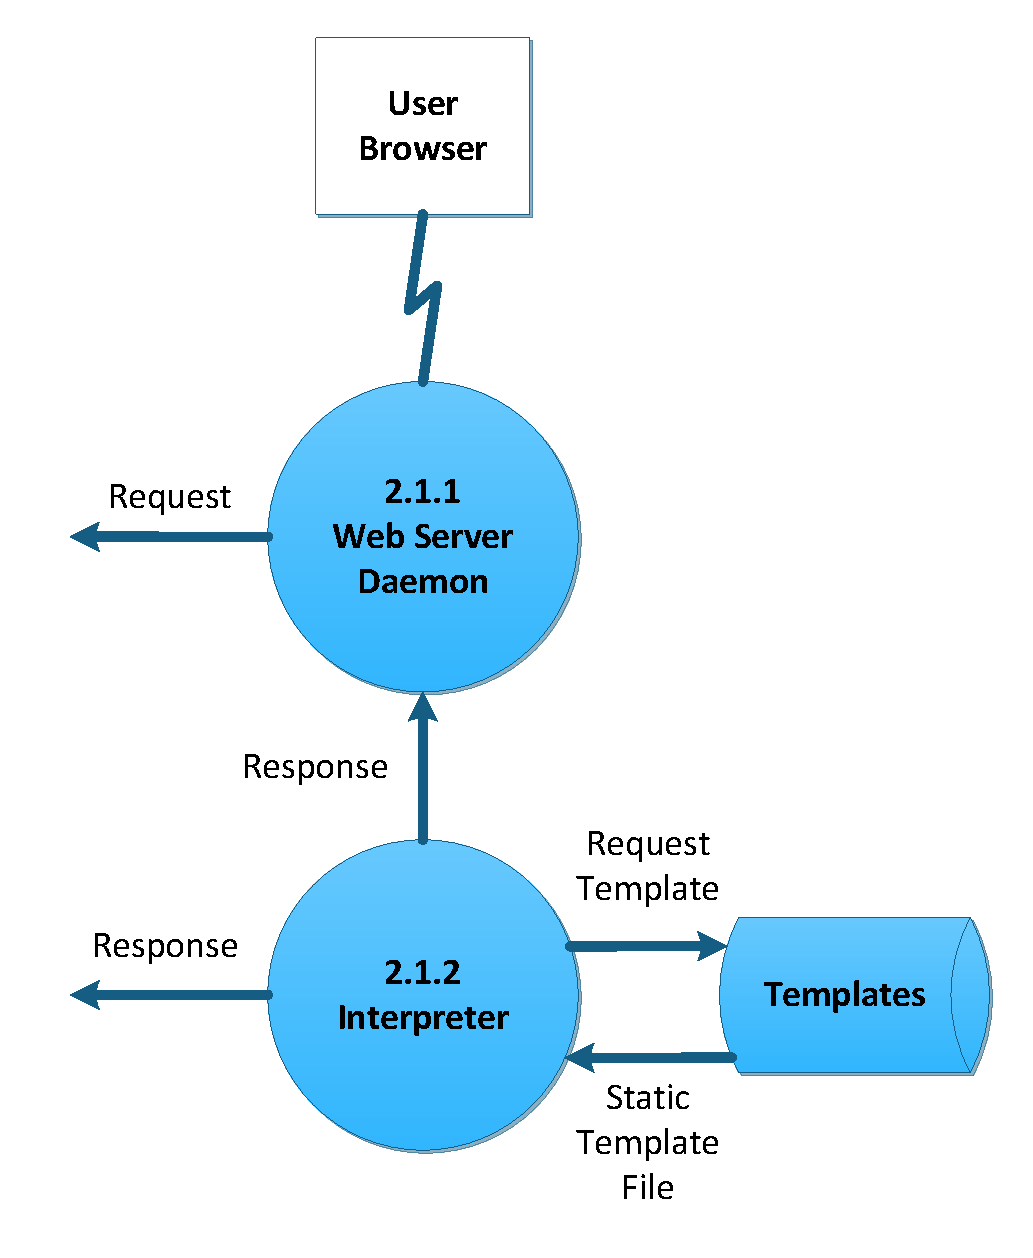
\includegraphics[scale=0.6]{DFD_level_2_1.pdf}
\caption{DFD Level 2.1}
\label{fig:DFD_level_2.1}
\end{figure}

\eject

\begin{figure}[h]
\centering
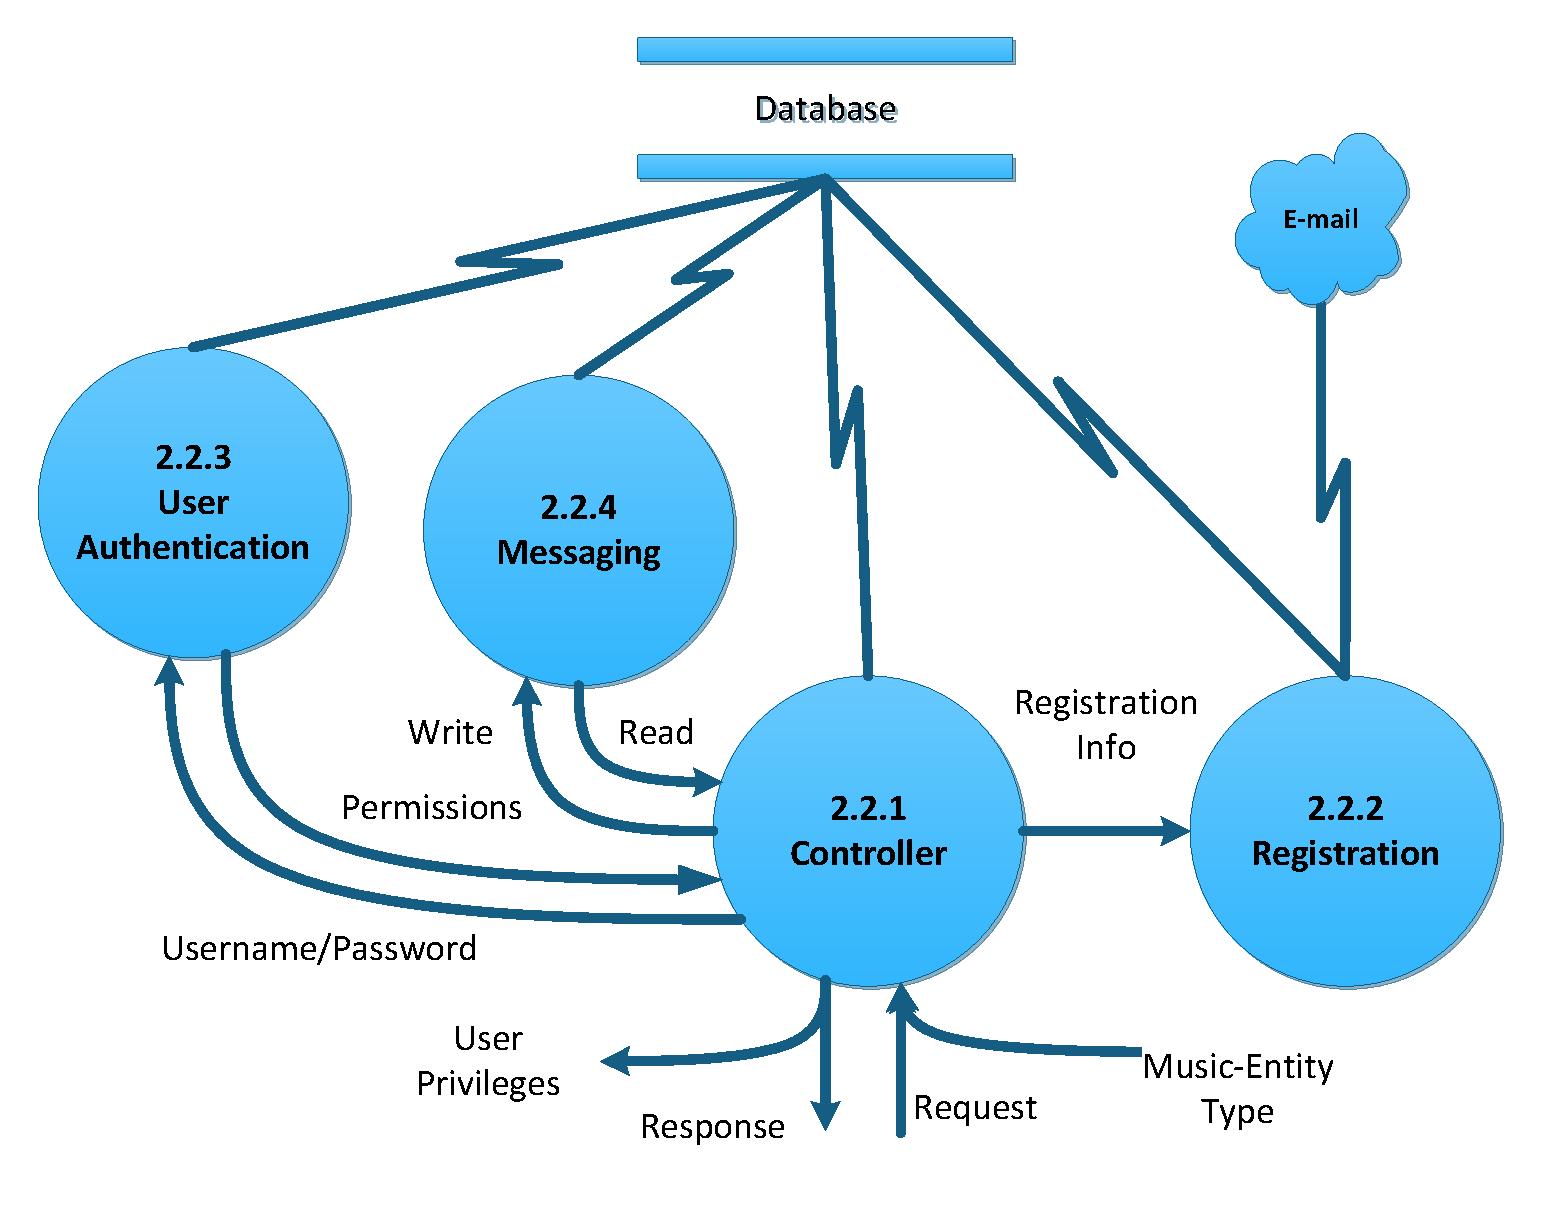
\includegraphics[scale=0.6]{DFD_level_2_2.pdf}
\caption{DFD Level 2.2}
\label{fig:DFD_level_2.2}
\end{figure}

\eject

\begin{figure}[h]
\centering
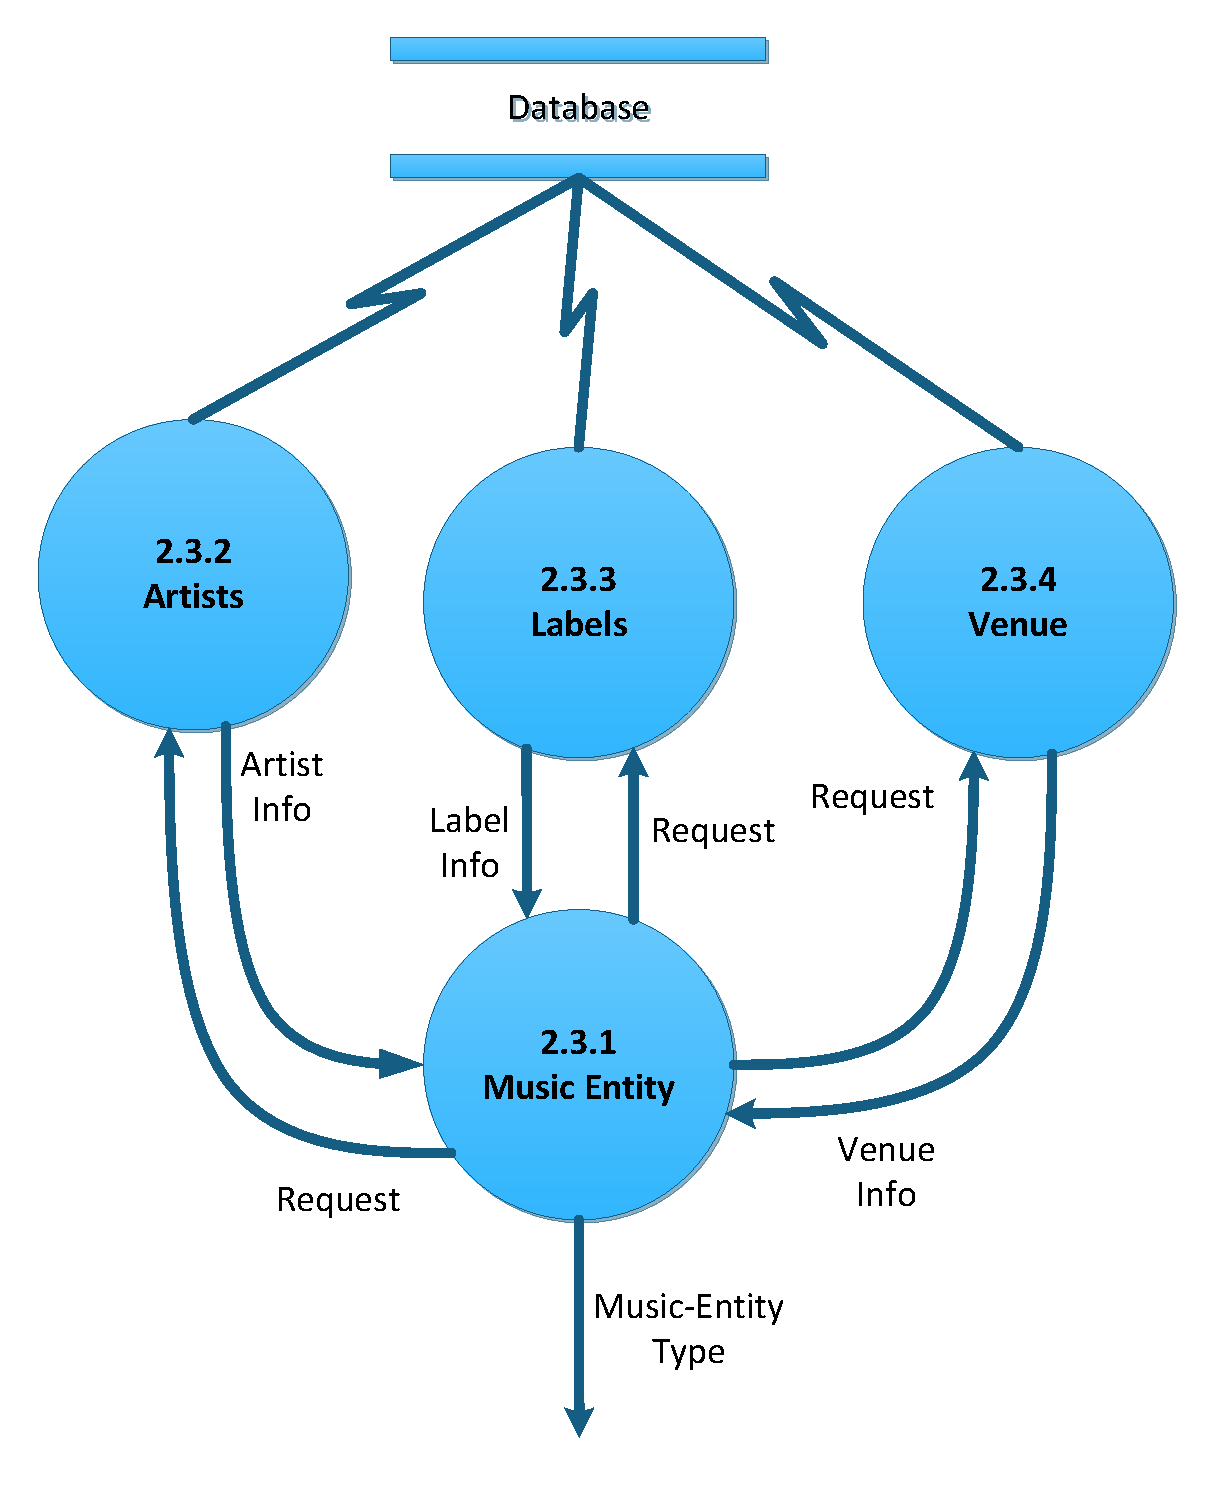
\includegraphics[scale=0.6]{DFD_level_2_3.pdf}
\caption{DFD Level 2.3}
\label{fig:DFD_level_2.3}
\end{figure}

\eject

 
\textcolor{section}{\Section{IM-Net Elements of Implementation}}

In this section (some of) the modules designed in Section 4 with requirements listed in Section 3 will be implemented initially at least at the level of pseudo code. Where possible, actual code will be provided. Each module is implemented in correspondence with the design sections defined in section 2 and responding to the requirements listed in its correlated sub-section in chapter 3.

\eject 

\textcolor{section}{\Section{IM-Net Test Plan}}

\textcolor{subsection}{\subsection{Introduction}}

In this section the testing methodology to be used to Verify and Validate each of the requirements listed in section 3.0 has been identified. At points some additional testing may be required and they shall be documented as an attachment to this document. 

The methodologies and testing strategies identified at this point include three major approaches with various variations to adapt to the IM-Net project:

\begin{enumerate}
\item  Testing using addition ad-hoc crated software including a correlation testing unit.

\item  Demonstration of the specified capability

\item  Inspection of the software code possibly using addition inspection techniques
\end{enumerate}

 
\textcolor{subsection}{\subsection{Functional Requirements Validation Matrix}}
The IM-Net Functional and Performance Requirements Validation Matrix is given below.
\eject 

\appendix

\textcolor{section}{\Section{Acronyms}}

\textbf{CSS} Cascading Style Sheets

\textbf{DFD} Data Flow Diagram

\textbf{IM-Net} Independent Music Network

\textbf{MVC} Model-View-Controller

\textbf{SQL} Structured Query Language

\textbf{W3C} World Wide Web Consortium

\textbf{XHTML} eXtensible HyperText Markup Language


\eject 
 
\textcolor{section}{\Section{Data Dictionary}}

\underline{Daemon}: A computer program that runs as a background process rather than being under control of a interactive user, typicaly started at boot time and serves the function of responding to network requests.

\underline{Django}: An open source web application framework, written in Python, which follows the Model-View-Controller architectural pattern.

\underline{Python}: A general-purpose, high-level programming language whose design philosophy emphasizes code readability and supports primarily, but not limited to, object-oriented, imperative and functional programming paradigms.

\end{document}
